\chapter{Anleitung für Docker starten}
\section{Docker starten}
\begin{enumerate}
    \item Verbinden mit \ac{hpc} 
    \item Unter \textit{/mnt/data/outside-data/} Ordner mit Namen Projekt anlegen für Studierenden (\textit{mkdir \textless Projektname\textgreater}) 
    \item Studierenden privaten Key vom Nutzer \textit{docker\_user} geben
    \item Studierende kopiert Daten auf \textit{/mnt/data/outside-data/} $\rightarrow$ die folgenden Schritte beziehen sich auf ein Windows Betriebssystem, für Linuxsysteme sind die ähnlichen Schritte nur die Berechtigungsschritte werden per \textit{chown 700 \textless user\textgreater \textless key\textgreater}
    
    \begin{enumerate}
        \item Studierende speichert Private Key auf PC ab
        \item Verbindung des PCs mit Mosbach VPN (Lehre Netz)
        \item Rechtsklick auf private Key im File Explorer $\rightarrow$ Properties $\rightarrow$ Sicherheit $\rightarrow$ erweitert $\rightarrow$ sollte Berechtigung sehen wie in \autoref{fig:berecht_1}
        \item klicken auf Vererbung Deaktivieren
        \item Hinzufügen klicken $\rightarrow$ SYSTEM suchen $\rightarrow$ Lese- und Execute und Schreibrechte geben $\rightarrow$ Ok klicken
        \item Hinzufügen klicken $\rightarrow$ \textit{\textless eigenen Nutzer\textgreater}  suchen $\rightarrow$ Lese- und Execute und Schreibrechte geben $\rightarrow$ Ok klicken
        \item danach sollte Berechtigung aussehen wie in \autoref{fig:berecht_2}
        \item Kommandozeile öffnen $\rightarrow$ wechseln in Directory wo Key legt
        \item Folgendes Kommando eingeben (alles eine Zeile)
        \begin{verbatim}
            scp -i <keyfile-name> -P 2022 <path-to-data>
            docker_user@193.197.11.229:/mnt/data/outside-data/
            <name-project>/  
        \end{verbatim}
        \begin{itemize}
            \item \textless path-to-data\textgreater $\rightarrow$ Pfad zur Base Directory $\rightarrow$ alles darin wird rüberkopiert
            \item \textless name-project\textgreater ist ein vorher angelegter Ordner, der den Namen des Projektes trägt, Password eingeben $\rightarrow$ wird von Herrn Müller übergeben
        \end{itemize} 
    \end{enumerate}
    \item Dockercontainer installieren und laufen lassen
\end{enumerate}

\begin{figure}
    \centering
    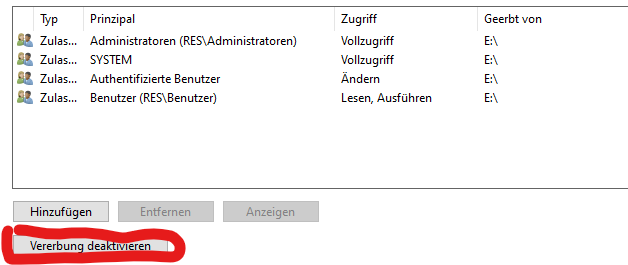
\includegraphics[width=8cm]{data/img/berechtigungen_1.png}
    \caption{Berechtigungen wie sie meistens voreingestellt sind durch Windows}
    \label{fig:berecht_1}
\end{figure}
\begin{figure}
    \centering
    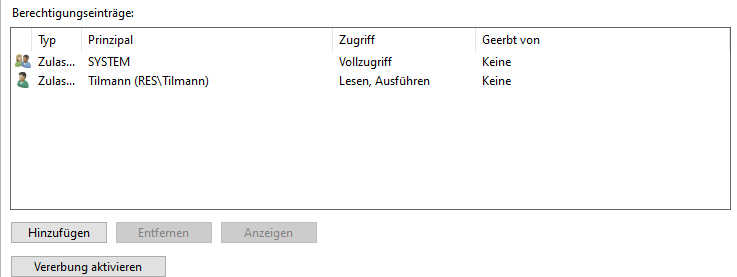
\includegraphics[width=8cm]{data/img/berechtigungen_2.png}
    \caption{Zielzustand Berechtigungen}
    \label{fig:berecht_2}
\end{figure}



\section{Docker YOLOv5 Container Setup und Vorbereitungen}

\textcolor{red}{\textbf{Wichtig:}} Die Umgebung mit \ac{yolo} und PyTorch ist schon aufgesetzt mit dem Dockercontainer der von Dockerhub gezogen wird. Insofern keine Änderungen am Algorithmus vorgenommen wurden, reicht dieser Container vollkommen aus und liefert alle nötigen Umgebungswerkzeuge.


\begin{enumerate}
    \item Entsprechenden Dockercontainer Pullen per Kommando: \textit{docker pull ultralytics/yolov5:latest} 
    \item eingeben Kommando unten (alles eine Zeile)
    \begin{verbatim}
        docker run --ipc=host -it --gpus all --memory="<memory-limit>"
        --cpus="<cpu-limit>" --network host -v 
        /mnt/data/outside-data/<projektname>/:/usr/src/datasets
        ultralytics/yolov5:latest
    \end{verbatim}
    \begin{itemize}
        \item \textless memory-limit\textgreater $\rightarrow$ Angabe wie viel RAM der Container nutzen darf $\rightarrow$ Vorzeichen wichtig: Gigabyte  $\rightarrow$ g / Megabyte $\rightarrow$ m
        \item \textless cpu-limit\textgreater $\rightarrow$ Angabe der CPU Begrenzung / wie viele CPUs dürfen maximal genutzt werden. Angabe als Gleitkommazahl: 2 CPUs entspräche 2.0
        \item sowohl die memory flag als auch cpu flag dürfen weg gelassen werden, dann läuft der Container mit den gesammten Resourcen des weg gelassenen Flag die der Rechner zur Verfügung stellt
        \item wenn der Container nicht die GPU bzw. der YOLO Algorithmus nutzen soll, muss die Flag: \textit{--gpus all} weggelassen werden
    \end{itemize}
    \item versichern Sie sich, dass die Daten unter \textit{/usr/src/datasets/} vorhanden sind
    \item geben sie \textit{exit} ein in die Kommandozeile 
    \item Eingeben des folgenden Kommandos:
    \begin{verbatim}
        docker start <cont-id>; docker exec <cont-id> <yolo-befehl> &
    \end{verbatim}
    \begin{itemize}
        \item  \textless cont-id\textgreater $\rightarrow$ ID des zu starteten containers. Ist einsehbar mit \textit{docker ps}
        \item \textless yolo-befehl\textgreater  Befehl zum Ausführen des Detektionsskriptes siehe \autoref{sec:yolo_train}
    \end{itemize}
\end{enumerate}

\subsection{YOLO Modell Trainieren}
\label{sec:yolo_train}

Für das Training des Modells muss in das  Base Directory von dem \ac{yolo}v5 Repository gewechselt werden oder der Befehl direkt abgesetzt werden siehe vorheriges Kapitel Schritt 5.

Für Training mit der Verbindung zum Docker Terminal ist es wichtig in dem Verzeichnis \textit{/usr/src/app} zu sein. Darin befindet sich die \textit{train.py}-Datei. Das Training kann durch folgenden Befehl gestartet werden:
\begin{verbatim}
    python train.py --img <size-of-img> --batch <size-of-batches> --epochs <epochs>
    --data <path-to-yaml> --weights <weights> [--device <device_numbers> ]
\end{verbatim}
\begin{itemize}
    \item \textless size-of-img\textgreater $\rightarrow$ definiert die Breite des Bildes in Pixel. Bei besonders kleinen Objekten (<3 Pixel) wird empfohlen die Originalauflösung zu nehmen. \textbf{Achtung:} Je höher der Pixelcount, desto höher der RAM / VRAM Verbrauch 
    \item \textless size-of-batch\textgreater $\rightarrow$  gibt an wie viele Bilder in einem Durchgang (Epoche) analysiert werden soll. Diese kann per Hand vorgegeben werden. Möglichkeit besteht des Abbruchs aufgrund unzureichender Ressourcen. Für dynamische Anpassung auf Basis zur Verfügung stehenden Ressourcen  $-1$ eingeben. Reserviert alle zur Verfügung stehenden Ressourcen.
    \item \textless epochs\textgreater $\rightarrow$  Angabe der Wiederholungsanzahl bzw. der Durchläufe. Für jede Epoche wird eine neue Batch an Images analysiert. Iteriert durch alle Bilder durch und fängt von vorne an bei Erreichen des Endes der Bilder
    \item \textless weights\textgreater $\rightarrow$ Angabe des Trainingsnetzwerkes. Für das Training gibt es 5 verschiedene Gewichte: Nano, Small, Medium, Large und XLarge. Für die jeweiligen Gewichte muss folgendes eingegeben werden. Es sei zu beachten, dass mit zunehmender größe die Rechendauer und der Platz an benötigten Arbeitsspeicher massiv zunimmt. Siehe \autoref{fig:yolo_mod_compar}
    \begin{itemize}
        \item Nano $\rightarrow $ \textit{yolov5n.pt}
        \item Small $\rightarrow $ \textit{yolov5s.pt}
        \item Medium $\rightarrow $ \textit{yolov5m.pt}
        \item Large $\rightarrow $ \textit{yolov5l.pt}
        \item XLarge $\rightarrow $ \textit{yolov5x.pt}
    \end{itemize}
    \item \textless device-numbers\textgreater $\rightarrow$ dies istt ein optionaler Parameter. Dieser gibt an welche GPUs genutzt werden sollen. Wenn kein GPUs genutzt wird muss der Parameter weg gelassen werden. Damit GPU(s) genutzt werden können müssen die Nummern der GPUs angegeben werden. Diese wird durch das Betriebssystem bestimmt. Wenn nur eine GPU vorhanden ist, ist dies i.d.R. 0. Damit wird der komplette VRAM der GPU genutzt. Voraussetzung dafür ist es, dass das NVIDIA CUDA Toolkit installiert ist und der GPU für den Docker freigeschaltet ist, was jedoch der default ist. Für mehrere GPUs einfach mit Kommata die GPUs auflisten. Für mehr Informationen die \textit{\href{https://github.com/ultralytics/yolov5/issues/475}{Dokumentation}} einsehen.
\end{itemize}
\begin{figure}
    \centering
    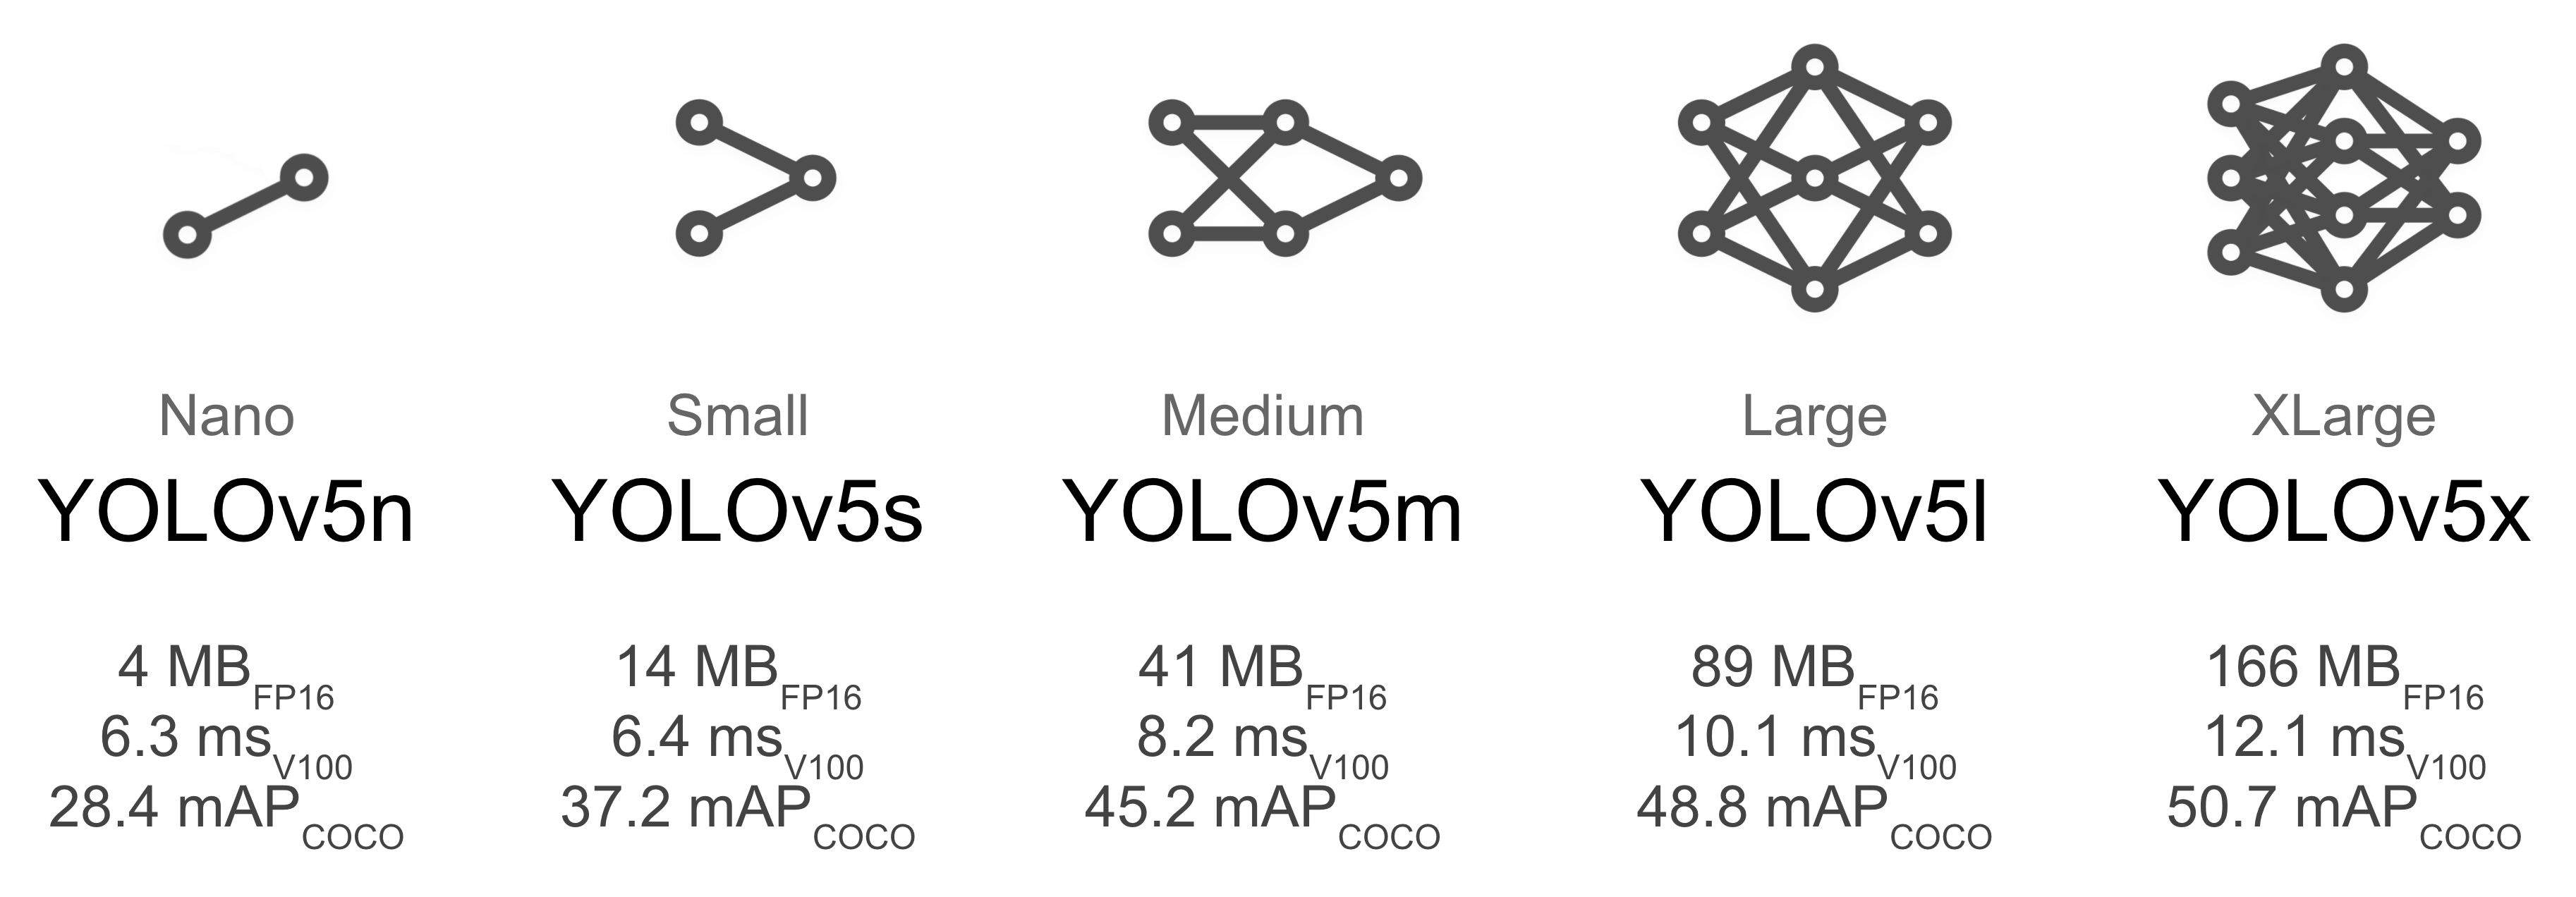
\includegraphics[width=12cm]{data/img/model_comparison.png}
    \caption{Vergleich der verschiedenen Modelle}
    \label{fig:yolo_mod_compar}
\end{figure}
\section{Den Docker Contaioner anschauen}
Dieser Abschnitt befasst sich damit wie man während des Laufes den Docker Container betreten kann ohne, dass der Trainingsprozess stoppt
\begin{enumerate}
    \item Docker Container anzeigen lassen mit \textit{docker ps}
    \item Konsole des Dockercontainer verbinden \textit{docker attach \textless cont\_id\textgreater} $\rightarrow$ damit wird die Konsolenausgabe des Dockercontainers mit der eigenen verbunden
    \item bei Verlassen erst \textit{Strg + P} und anschließend \textit{Strg + Q} drücken 
\end{enumerate}

\section{Docker Container stoppen und löschen}
Zum Stoppen des Containers kann der folgende Befehl gesetzt werden:
\begin{verbatim}
    docker stop <container_name>
\end{verbatim}
Der \textless container\_name\textgreater kann durch den Befehl \textit{docker ps} angezeigt werden. Dabei wird in der letzten Spalte der Containername angezeigt und in der ersten Spalte die id. \textit{docker stop} nutzt die ID des Docker Containers.

Mit dem Befehl \textit{docker rm \textless container\_id\textgreater} kann dann der Container gelöscht werden 